\documentclass[
	% -- opções da classe memoir --
	12pt,				% tamanho da fonte
	openright,			% capítulos começam em pág ímpar (insere página vazia caso preciso)
	oneside,			% para impressão em verso e anverso. Oposto a oneside
	a4paper,			% tamanho do papel.
	% -- opções da classe abntex2 --
	chapter=TITLE,		% títulos de capítulos convertidos em letras maiúsculas
	section=TITLE,		% títulos de seções convertidos em letras maiúsculas
	%subsection=TITLE,	% títulos de subseções convertidos em letras maiúsculas
	%subsubsection=TITLE,% títulos de subsubseções convertidos em letras maiúsculas
	% -- opções do pacote babel --
	english,			% idioma adicional para hifenização
	brazil				% o último idioma é o principal do documento
	]{abntex2}

% ---
% Pacotes básicos
% ---
\usepackage{times}			    % Usa a fonte ADOBE Times
\usepackage[T1]{fontenc}		% Selecao de codigos de fonte.
\usepackage[utf8]{inputenc}		% Codificacao do documento (conversão automática dos acentos)
\usepackage{lastpage}			% Usado pela Ficha catalográfica
\usepackage{indentfirst}		% Indenta o primeiro parágrafo de cada seção.
\usepackage{color}				% Controle das cores
\usepackage{graphicx}			% Inclusão de gráficos
\usepackage{microtype} 			% para melhorias de justificação
\usepackage{mathtools}          % para uso de funções matemáticas
\usepackage{xfrac}              % para usar frações com \
%\usepackage{multirow}           % Usado para mesclar linhas e colunas de uma tabela
% ---


% ---
% Pacotes de citações
% ---
%\usepackage[brazilian,hyperpageref]{backref}	 % Paginas com as citações na bibl
\usepackage[alf,bibjustif]{abntex2cite}	% Citações padrão ABNT

% ---
% CONFIGURAÇÕES DE PACOTES
% ---

% ---
% Configurações do pacote backref
% Usado sem a opção hyperpageref de backref
%\renewcommand{\backrefpagesname}{Citado na(s) página(s):~}
%% Texto padrão antes do número das páginas
%\renewcommand{\backref}{}
%% Define os textos da citação
%\renewcommand*{\backrefalt}[4]{
%	\ifcase #1 %
%		Nenhuma citação no texto.%
%	\or
%		Citado na página #2.%
%	\else
%		Citado #1 vezes nas páginas #2.%
%	\fi}%
% ---
\graphicspath{ {./images/} }
% Fontes dos títulos e seções (no texto e no sumário, respectivamente)
\renewcommand{\ABNTEXchapterfont}{\bfseries}
\renewcommand{\ABNTEXchapterfontsize}{\normalsize}
%
\renewcommand{\ABNTEXsectionfont}{\normalfont}
\renewcommand{\ABNTEXsectionfontsize}{\normalsize}
%
\renewcommand{\ABNTEXsubsectionfont}{\bfseries}
\renewcommand{\ABNTEXsubsectionfontsize}{\normalsize}
%
\renewcommand{\ABNTEXsubsubsectionfont}{\normalfont}
\renewcommand{\ABNTEXsubsubsectionfontsize}{\normalsize}

%
\renewcommand{\cftchapterfont}{\normalfont\bfseries}
\renewcommand{\cftchapterpagefont}{\normalsize}
%
\renewcommand{\cftsectionfont}{\normalfont\uppercase}
\renewcommand{\cftsectionpagefont}{\normalsize}
%
\renewcommand{\cftsubsectionfont}{\normalsize\bfseries}
\renewcommand{\cftsubsectionpagefont}{\normalsize}
%
\renewcommand{\cftsubsubsectionfont}{\normalfont}
\renewcommand{\cftsubsubsectionpagefont}{\normalsize}

%Substitui o texto "Referências" por "REFERÊNCIAS" no sumário
\addto\captionsbrazil{%
  \renewcommand{\bibname}%
    {\uppercase{Referências}}%
}

% ---
% Informações de dados para CAPA e FOLHA DE ROSTO
% ---
\titulo{ATIVIDADE 1 \\ ROBO SEGUIDOR DE PAREDE}
\autor{David Ferrari}
\local{Salvador, Bahia}
\data{2021}
\instituicao{Universidade Federal da Bahia}

% Configurações de aparência do PDF final

% alterando o aspecto da cor azul
\definecolor{blue}{RGB}{41,5,195}

% informações do PDF
\makeatletter
\hypersetup{
     	%pagebackref=true,
		pdftitle={\@title},
		pdfauthor={\@author},
    	pdfsubject={\imprimirpreambulo},
	    pdfcreator={LaTeX with abnTeX2},
%	    Coloque suas keyword aqui!!
		pdfkeywords={keyword 1}{keyword 2}{keyword 3}{keyword 4},
		colorlinks=true,       		% false: boxed links; true: colored links
    	linkcolor=black,          	% color of internal links
    	citecolor=black,        		% color of links to bibliography
    	filecolor=black,      		% color of file links
		urlcolor=black,
		bookmarksdepth=4
}
\makeatother
% ---

% ---
% Espaçamentos entre linhas e parágrafos
% ---

% O tamanho do parágrafo é dado por:
\setlength{\parindent}{1.3cm}

% Controle do espaçamento entre um parágrafo e outro:
\setlength{\parskip}{0.2cm}  % tente também \onelineskip

% Cotrole do espaçamento entre o título de um capítulo e o ínicio do seu texto referente
% NBR 14724:2011 - "Os títulos das seções primárias devem começar em página ímpar (anverso), na parte superior da mancha gráfica e ser separados do texto que os sucede por um espaço entre as linhas de 1,5."
\setlength\afterchapskip{18pt}

\setlength\aftersecskip{18pt}

\setlength\aftersubsecskip{18pt}

\setlength\aftersubsubsecskip{18pt}

% ---
% compila o indice
% ---
\makeindex
% ---

\begin{document}

% Retira espaço extra obsoleto entre as frases.
\frenchspacing

% ----------------------------------------------------------
% ELEMENTOS PRÉ-TEXTUAIS
% ----------------------------------------------------------
\pretextual

% ---
% Capa
% ---
\renewcommand{\imprimircapa}{
 \begin{capa}
  \center
  \includegraphics[scale=1]{Brasao_UFBA.png}  \\
  {\bfseries\Large\MakeUppercase\imprimirinstituicao}
   \\
   \vfill
 {\bfseries\large\MakeUppercase\imprimirautor}
 \vfill
 {\bfseries\Large\MakeUppercase\imprimirtitulo}
 \vfill
 {\large\imprimirlocal}
 \par
 {\large\imprimirdata}
 \vspace*{1cm}
 \end{capa}
 }
\imprimircapa
% ---

% --- Sumário --- %
\pdfbookmark[0]{\contentsname}{toc}
\tableofcontents*
\cleardoublepage


% ----------------------------------------------------------
% ELEMENTOS TEXTUAIS
% ----------------------------------------------------------

\textual  %Indica que aqui começam os elementos textuais do documento, isso cria, a partir daqui a numeração de páginas!

%Retira indicação de capítulo e seção no cabeçalho da página deixando apenas a numeração de página.
\pagestyle{simple}
\section{Introdução ao problema}
Nesse problema temos um robô em um mundo matricial onde o mesmo tem sensores H(Head) e L(Left) permitindo que o robô "enxergue" paredes imediante a sua frente e paredes a sua esquerda, o objetivo é desenvolver um robô capaz de seguir paredes posicionadas a esquerda do mesmo.


\section{Diagrama de estados e tabela de transição de estados}
Para construção do diagrama de estados e posteriormente tabela de transição de estados do sistema, considerei os dois estados, S0 significando o robô em uma parede(seguindo a mesma) e o estado S1 que seria o robô fora de uma parede(procurando uma), respeitando as entradas H e L e criando 2 saídas A(avanço) e R(rotação) temos o seguinte diagrama de estados: \\
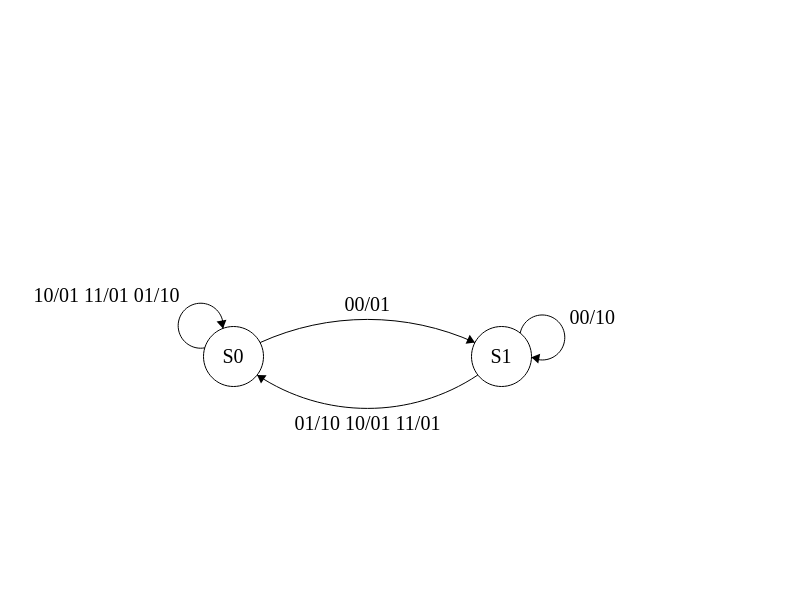
\includegraphics[scale=0.55]{diagrama-de-estados.png}
\\

Este diagrama de estados por sua vez gera a seguinte tabela de transição de estados:

\begin{tabular}{ |c|c|c|c|c|c| }
\hline
S & H & L & SF & A & R \\
\hline
\multirow{S0} & 0 & 0 & 1 & 0 & 1 \\
& 0 & 1 & 0 & 1 & 0 \\
& 1 & 0 & 0 & 0 & 1 \\
& 1 & 1 & 0 & 0 & 1 \\
\hline
\multirow{S1} & 0 & 0 & 1 & 1 & 0 \\
& 0 & 1 & 0 & 1 & 0 \\
& 1 & 0 & 0 & 0 & 1 \\
& 1 & 1 & 0 & 0 & 1 \\
\hline
\end{tabular}

Dessa forma o robô estando conectado a uma parede permanece seguindo-a vide situação 01/10 no estado S0, e quando o mesmo encontra uma curva, situação 00/01 transita para estado fora da parede e rotaciona a esquerda, após isso no estado S1 o mesmo efetua o movimento para frente e passa a procurar uma parede que possa ser seguida, transicionando novamente para o estado S0.

O funcionamento do robô é simples e pode ser iniciado em qualquer estado seja ele o S0 colocando o robô já colado a uma parede, quanto colocando o robô numa posição livre(sem paredes a vista do robô).


%Sua dissertação aqui!
%Recomendo criar arquivos para cada capítulo e chamá-los aqui assim:
\section{Circuito e simulação temporal}
Por fim com diagrama e tabela de transição de estados em mãos basta construir o circuito, este circuito só necessita de 1 flip-flop do tipo D, sendo o valor 0 estado S0 e o valor 1 estado S1:
\\
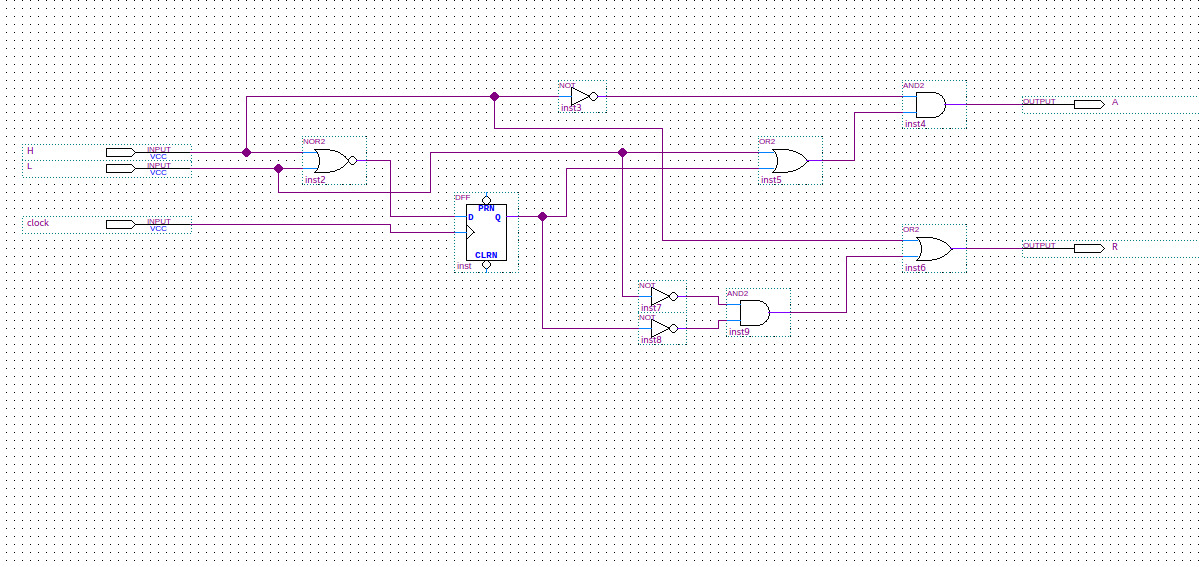
\includegraphics[scale=0.43]{images/circuito.jpeg}
\\ \\
\\
\\
A simulação nos traz exatamente o esperado segundo o diagrama de estado anteriormente visto:
\\ \\
\includegraphics[scale=0.38]{images/analise-temporal-maximizada.jpeg}
\\
Representação na ordem seriam, clock verde, H verde, L verde, saída A azul, saída R vermelho e estado em branco.
% ----------------------------------------------------------
% ELEMENTOS PÓS-TEXTUAIS
% ----------------------------------------------------------
\postextual
% ----------------------------------------------------------

% ----------------------------------------------------------
% Referências bibliográficas
% ----------------------------------------------------------
%\bibliography{refs-dissertacao_v1}

\end{document}
